\chapter{Lezione 3 - Approccio quantitativo al progetto e all'analisi. Parte 3}

Continuiamo l'argomento dell'approccio quantitativo al progetto e all'analisi, al progetto e all'analisi di architetture di elaborazione.

\FloatBarrier
\begin{figure}[H]
  \centering
  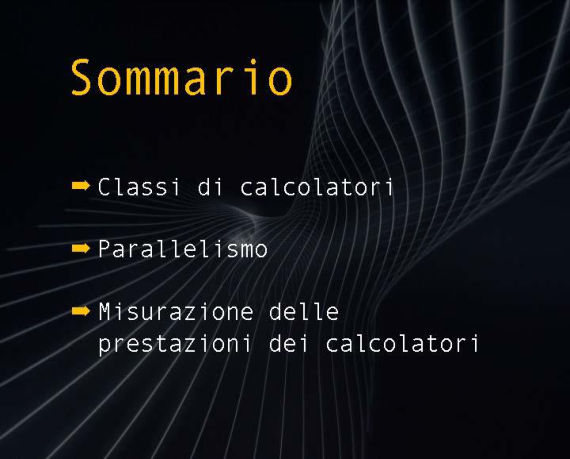
\includegraphics[width=0.40\textwidth,
                    trim=40 80 10 40, % L B R T
                    clip]
                    {images/Lez03_p01_fig_02.png}
  \caption{Sommario}
  \label{fig:Lez03_p01_fig_02}
\end{figure}
\FloatBarrier
\noindent

Fra le classi di calcolatori vi faccio un rapido richiamo al fine di avere un linguaggio comune.

\FloatBarrier
\begin{figure}[H]
  \centering
  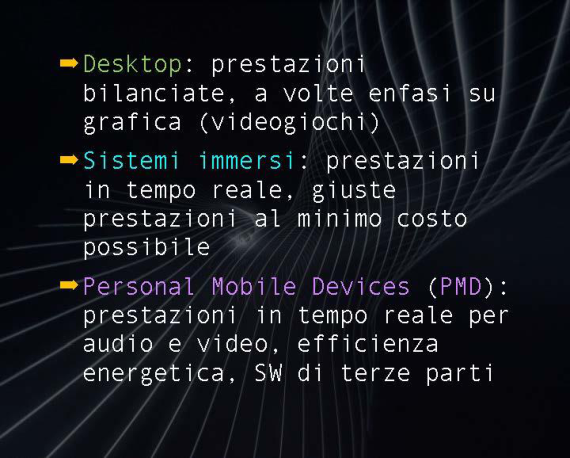
\includegraphics[width=0.40\textwidth,
                    trim=40 50 10 40, % L B R T
                    clip]
                    {images/Lez03_p01_fig_04.png}
  \caption{Sommario}
  \label{fig:Lez03_p01_fig_04}
\end{figure}
\FloatBarrier
\noindent

Definiamo desktop, quei calcolatori da tavolo, quelli che storicamente sono stati personal computers, sono caratterizzati da prestazioni bilanciate a volte c'è enfasi sulla grafica, cioè sui videogiochi.
Questo è il classico computer da casa, da ufficio, oramai un'architettura multicore, per i motivi che vi ho raccontato nelle lezioni precedenti.
Spesso è un'architettura multicore, ma più che i core del microprocessore, quelli che più interessano sono gli elementi grafici, perché spesso vengono utilizzati come delle piattaforme di gioco o per altre attività multimediali nelle mura domestiche.
Spesso è uno spreco di risorse di calcoli e comunque la definizione di prestazioni bilanciate significa che né si esaltano le prestazioni, né si esalta il risparmio di potenza, perché nel primo caso non è necessario avere prestazioni di calcolo necessariamente al massimo, nel secondo caso essendo dei dispositivi attaccati all'alimentazione di rete e generalmente anche abbastanza spaziose all'interno è possibile utilizzare come metodo di raffeddamento con radiatori e ventole che possono tranquillamente rimuovere potenza nell'ordine del centinaio di watt.
Se ricordate il grafico della lezione precedente, più o meno quelle sono le potenze.
Siamo che al momento i desktop di ultima generazione hanno un TDP attorno ai 77 watt.
Come vi ho detto questa è stata una potenza che è scesa rispetto ai picchi di pochi anni fa, ma comunque si tratta di potenze non completamente trascurabili e come se andate a aprire una scatola vi accorgete immediatamente che internamente vi sono anche dei corposi radiatori e delle ventole montate.
Se vi volete sbizzarrire nel vedere l'andamento delle potenze e delle temperature ci sono delle utility di sistema o di terze parti spesso che vi consentono di farlo.
È molto illuminante vedere questo.
Un esempio sotto Windows potrebbe essere CPU Z che vi permette di vedere molte di queste caratteristiche.
Capire cosa si intende per prestazioni bilanciate, a quanto va la frequenza del clock, a che tensione lavora il processore e generalmente la potenza che esso dissipa.

Altri sistemi sono i cosiddetti sistemi immersi che è una brutta traduzione dell'inglese embedded systems e sono tutti quei sistemi caratterizzati generalmente da prestazioni in tempo reale, giuste prestazioni al minimo costo possibile.
Ovviamente giusto è un termine soggettivo, quello che intendiamo con questo aggettivo è quello di dire che i sistemi embedded, li chiameremo sempre embedded systems o sistemi embedded perché il sistema è immerso in un termine molto poco utilizzato nella comunità, intendiamo quei sistemi che sono dedicati a una particolare funzione.
Embedded system può essere qualunque cosa, dal controllore della vostra lavatrice a un sistema come un router di rete, in qualche modo anche a una console per videogiochi, anche se una console per videogiochi sia un desktop o un sistema immerso è un po' grigio come intervallo perché molte funzionalità di queste console sono di fatto quasi equivalenti a quelle di un desktop anche se è un po' meno general purpose, cioè ha uso meno generale. Però ad esempio con una molte console potete navigare, vedere filmati, vedere DVD e così via.
La cosa caratteristica che descrive i sistemi immersi è che tecnicamente sono dei sistemi chiusi, cioè non sono modificabili o non è possibile caricare su essi dei programmi prodotti da soggetti diversi dal prodotto del sistema immerso tal quale, per questo vi ho detto che anche ad esempio una console è un po' grigio perché alcune cose possono girare e non necessariamente tutto.

Una particolare categoria di sistemi embedded possono essere i cosiddetti personal mobile devices, le caratteristiche più importati sono le prestazioni in tempo reale per audio e video, l'efficienza energetica e la possibilità di far girare software di terze parti.
L'ultima di queste caratteristiche, la possibilità di far girare software di terze parti, li rende sostanzialmente diversi dai sistemi embedded di tipo convenzionale.
In qualche modo sono al confine fra un personal computer di tipo portatile e un sistema immerso. La caratteristica fondamentale che possono far girare i software di terze parti è che hanno delle innovative modalità di input e di output che abbiamo discusso nelle due lezioni fa, ma in tutta sostanza sono dei calcolatori embedded che hanno un insieme di funzionalità abbastanza ottimizzate per uno specifico impiego.
Sono un po' meno general purpose anche se in alcuni di essi è possibile utilizzare delle porte esterne, per esempio una porta USB per ad esempio pilotare appositi ulteriori dispositivi o lo si può fare anche in modalità wireless.
Fra i personal mobile device vi ricordo quelli che utilizzate comunemente, gli smartphones, i tablets e i loro ibridi, cioè i phablets, quella categoria di piccoli tablet o grandi smartphone, indicativamente attorno ai 5-6 pollici di diagonale che ultimamente stanno prendendo abbastanza piede e che al crescere delle dimensioni vedono sempre meno critiche le esigenze, i vincoli di natura di efficienza energetica, ma comunque qualunque utente vorrebbe poter utilizzare liberamente questo tipo di PMD nell'arco di almeno un'intera giornata e vi accorgete spesso che quando sono più compatti questo risulta particolarmente difficoltoso.

%07:12

\FloatBarrier
\begin{figure}[H]
  \centering
  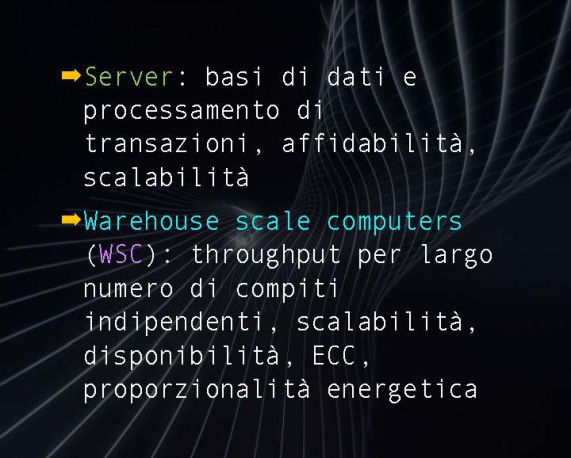
\includegraphics[width=0.40\textwidth,
                    trim=40 80 10 40, % L B R T
                    clip]
                    {images/Lez03_p01_fig_05.png}
  \caption{Sommario}
  \label{fig:Lez03_p01_fig_05}
\end{figure}
\FloatBarrier
\noindent

A un altro estremo troviamo i server, sono utilizzati per basi di dati e per processamento di transazioni caratterizzati da affidabilità e scalabilità.
Nel caso dei server immaginate una transazione di una banca, l'affidabilità è fondamentale, ma anche la scalabilità perché se aumentano il numero di sportelli di Bancomat il sistema deve poter essere scalabile.
Una specie di estremo dei server è il cosiddetto warehouse scale computers, cioè quei computer di grande dimensione interconnessi per cui il throughput per un largo numero di compiti indipendenti è una caratteristica fondamentale, rimane ancora la scalabilità, la disponibilità del sistema, vi ho fatto l'esempio della transazione di natalizia e di acquisto, la correzione d'errore perché non si vuole per esempio che in una transazione vi sia un errore nella registrazione per esempio del conto su cui accreditare l'attività e la cosiddetta proporzionalità energetica che è una caratteristica annessa alla scalabilità.

Cosa si intende per proporzionalità energetica?
Si intende che se si aumenta per esempio del 10\% la capacità di calcolare e di gestire transazioni, il consumo di energia non deve aumentare di più del 10%.
Questo è molto importante perché chiaramente il costo energetico sia in termini di bolletta energetica per far funzionare le architetture di elaborazione, sia per smaltire il calore, sono spesso una voce molto importante del costo complessivo della gestione di queste warehouse scale computers, cioè questi sono computer alla fine interconnessi fra loro ma in un modo scalabile, in modo proporzionalmente energetico, in maniera tale che manifesti un elevato tasso di disponibilità perché la perdita ad esempio di un singolo nodo non deve pregiudicare in nessun modo il funzionamento complessivo della piattaforma.
Vi faccio i classici esempi, Amazon, Google, Facebook, non volete che sia a un certo punto una delle macchine che fa le transazioni abbia un danno, una ruttura di un disco, la bruciatura di un processore, di uno zoccolo di memoria e così via, non vi potete aspettare che tutta Facebook smetta di funzionare, quindi in quei casi è necessario disegnare queste warehouse scale computers opportunamente.
È anche interessante considerare il fatto che ormai molte di queste warehouse scale computers non vengono più poste presso la sede dell'azienda stessa ma in locazioni ambientalmente favorevoli.

Quali sono le locazioni ambientalmente favorevoli?
Quelle dove l'energia elettrica costa poco e quelle dove è possibile facilmente smaltire il calore e quindi tipicamente l'Islanda o il nord degli Stati Uniti o del Canada nel caso in cui le aziende preferiscono mantenere nello stesso Paese dati sensibili.
Considerate che la gestione di questi dati è molto importante, vi sono anche delle importanti agenzie di intelligence che spesso accedono senza che voi sappiate, quindi state molto cauti su quello che andate a mettere sui siti social, su quello che andate a scrivere perché c'è sempre qualcuno, qualche intruso che ascolta.

Siccome un sistema consuma potenza è importante pagare una bolletta energetica più economica ed è importante per esempio semplicemente ventilare senza dover utilizzare dei condizionatori.
Immaginate la differenza fra dove smaltire il calore, per esempio nel sud degli Stati Uniti, in Sicilia visto che siamo in Italia, oppure smaltirlo nel nord della Scandinavia, in Islanda, in Greenlandia, cioè in quei posti dove l'aria è sempre abbastanza fresca anche nel caso di massima temperatura.
I casi esempio dell'Islanda sono anche legati al fatto che l'energia elettrica è a buon mercato grazie al geotermico.
Altri paesi, esempio il Canada, hanno una ampia disponibilità di idroelettrico, quindi in certi paesi l'energia elettrica costa meno, quindi in quei paesi è conveniente mettere dei servizi fortemente energivori come possono essere per esempio le warehouse scale computers dove ci sono spesso potenze di molte decine di megawatt impiegate per la gestione della struttura. Provate a fare un conto sulla bolletta.

\subsubsection{Supercomputer}

\FloatBarrier
\begin{figure}[H]
  \centering
  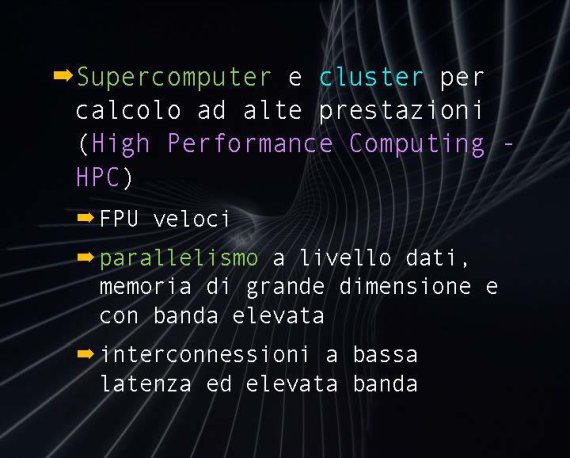
\includegraphics[width=0.40\textwidth,
                    trim=40 80 10 40, % L B R T
                    clip]
                    {images/Lez03_p01_fig_06.png}
  \caption{Sommario}
  \label{fig:Lez03_p01_fig_06}
\end{figure}
\FloatBarrier
\noindent
%12:28
Un caso particolare di macchine di calcolo sono i supercomputer e i cluster per calcolo ad alte prestazioni, quello che in inglese si chiama high performance computing o HPC che abbiamo già utilizzato precedentemente come acronimo.
La caratteristica di questi consiste nel cercare di eseguire molte operazioni, esempio quindi servono delle FPU  veloci, cioè delle floating point unit veloci, quindi parallelismo a livello dati, memoria di grande dimensione e con banda elevata e inoltre interconnessioni a bassa latenza ed elevata a banda.
Con questo vi do un piccolo spunto per la riflessione e vi invito a pensare in quale classe di calcolatori la latenza delle comunicazioni fra core e nell'accesso alla memoria è più critica e perché.

\subsubsection{Parallelismo}

\FloatBarrier
\begin{figure}[H]
  \centering
  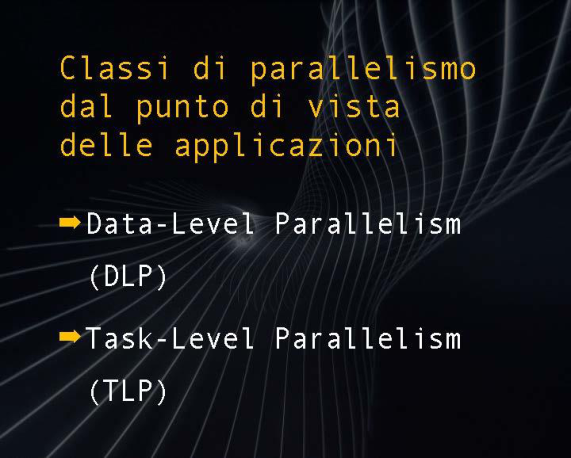
\includegraphics[width=0.40\textwidth,
                    trim=40 80 10 40, % L B R T
                    clip]
                    {images/Lez03_p02_fig_03.png}
  \caption{Parallelismo}
  \label{fig:Lez03_p02_fig_03}
\end{figure}
\FloatBarrier
\noindent

Prossimo argomento è il concetto di parallelismo (fig. \ref{fig:Lez03_p02_fig_03})

Le classi di parallelismo dal punto di vista delle applicazioni possono essere divise in quelle che vengono chiamate in inglese il data level parallelism, cioè il parallelismo a livello di dati o il task level parallelism, cioè il parallelismo a livello di compito. Questo dal punto di vista delle applicazioni.

\FloatBarrier
\begin{figure}[H]
  \centering
  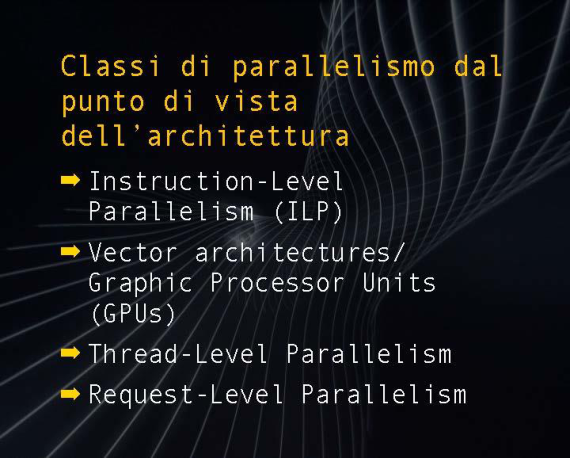
\includegraphics[width=0.40\textwidth,
                    trim=40 30 10 40, % L B R T
                    clip]
                    {images/Lez03_p02_fig_04.png}
  \caption{Parallelismo}
  \label{fig:Lez03_p02_fig_04}
\end{figure}
\FloatBarrier
\noindent

Le classi di parallelismo invece dal punto di vista dell'architettura vengono classificate in instruction level parallelism, quindi a livello di istruzione.
Fra queste consideriamo le unità vettoriali o unità di processamento grafico, graphic processor units, quelle che voi conoscete come GPU, per fare calcoli grafici ma anche per fare calcoli numerici importanti dove l'elevato livello di parallelismo può consentire accelerazioni notevoli rispetto ai processori di tipo general purpose.
Il cosiddetto thread level parallelism, cioè quello a livello di trama.
Parleremo di questo livello di parallelismo molto nel dettaglio nelle lezioni più successive.

Infine il cosiddetto request level parallelism, cioè il parallelismo a livello di richiesta della transazione.

\subsubsection{Tassonomia di Flynn}

\FloatBarrier
\begin{figure}[H]
  \centering
  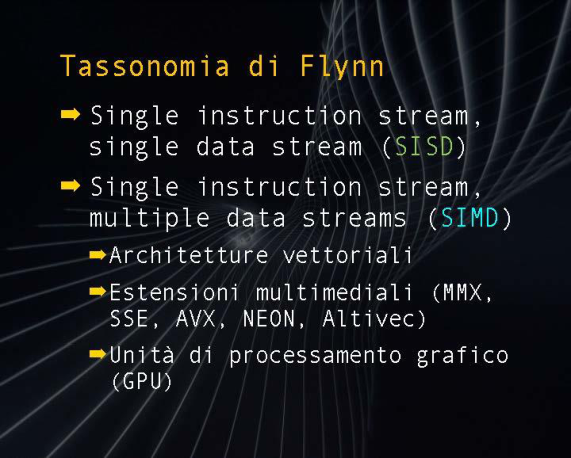
\includegraphics[width=0.40\textwidth,
                    trim=40 80 10 40, % L B R T
                    clip]
                    {images/Lez03_p02_fig_05.png}
  \caption{Tassonomia di Flynn}
  \label{fig:Lez03_p02_fig_05}
\end{figure}
\FloatBarrier
\noindent

Vi introduco una definizione, quella che viene chiamata tassonomia di Flynn.
Questo approccio fu introdotto ormai parecchi decenni fa ma la comunità scientifica e tecnica la usa con grande frequenza.
Consideriamo le cosiddette single instruction stream, single data stream o SISD, cioè un'architettura che svolge operazioni su un singolo flusso di istruzioni, su un singolo flusso di dati.
Cioè il classico calcolatore che abbiamo visto nei corsi del primo livello, c'è una sola istruzione alla volta senza pipeline, senza parallelismi, senza nulla di particolare, cioè c'è un dato, c'è un flusso di istruzioni.

La fase successiva è il cosiddetto single instruction stream, multiple data stream, cioè via un singolo flusso di istruzioni ma quelle istruzioni agisce su un insieme di dati.
Per esempio una delle cose più semplici è un'architettura vettoriale dove ad esempio facciamo una add fra gli elementi di un vettore e gli elementi di un altro vettore, in questo caso immaginiamo ad esempio di avere una cosa molto semplice, un vettore fatto di 4 parole di interi che viene sommato su un altro vettore di 4 parole di interi.
L'istruzione è un add vettoriale in cui parola per parola vengono sommate e vengono messe in un terzo registro, anch'esso in questo caso della dimensione di 4 parole 128 bit, il che consente con una singola istruzione, un singolo flusso di istruzioni di eseguire istruzioni su più flussi di dati in parallelo.

Esistono molte implementazioni di questa architettura SIMD nelle estensioni multimediali, ad esempio nell'intel le prime MMX, le varie versioni di SE, le più moderne AVX, nell'ARM il neon, nell'architettura Power l'Altivec, tutte unità con varie versioni, con vari livelli di parallelismo che agiscono su flussi paralleli, da un minimo di 64 bit dell'MMX fino alle versioni più avanzate dell'AVX2 che agiscono su 512 bit.

Questo consente di aumentare notevolmente il throughput di esecuzione senza aumentare né la quantità di istruzioni, quindi la dimensione del codice, né in linea di principio aumentare i tempi, però ovviamente nulla viene esattamente a costo zero.

Un altro tipo di esempio di SIMD sono le unità di processamento grafico dove le operazioni vengono fatte su unità di memoria che rappresentano i colori dei pixel, passeremo anche su questo più avanti.

\FloatBarrier
\begin{figure}[H]
  \centering
  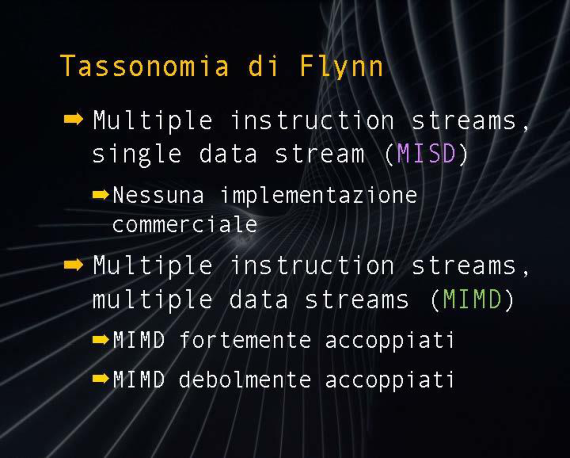
\includegraphics[width=0.40\textwidth,
                    trim=40 40 10 40, % L B R T
                    clip]
                    {images/Lez03_p02_fig_06.png}
  \caption{Tassonomia di Flynn I}
  \label{fig:Lez03_p02_fig_06}
\end{figure}
\FloatBarrier
\noindent


Procedendo nella tassomia di Flynn esistono i cosiddetti multiple instruction stream, single data stream o MISD anche se di questo non vi è nessuna implementazione commerciale, è troppo pesante da realizzare, i vantaggi sono modesti rispetto ad andare nella massima generalizzazione cioè il multiple instruction stream, multiple data stream o MIMD che può essere classificato in MIMD fortemente accoppiati o MIMD debolmente accoppiati.
Su queste classificazioni torneremo più avanti, notate che in questo caso è un'architettura parallela che fa cose diverse su flussi di dati diversi e li fa in simultanea.
Non è semplice ovviamente da gestire, l'esempio che vi ho fatto di una semplice architettura vettoriale è chiaramente quello più semplice e più intuitivo.
Con questo vi do un altro spunto per la riflessione e vi invito a riflettere se i processori in multicore possono sempre essere considerati più veloci e secondo voi quali sono gli elementi che limitano l'aumento delle prestazioni nei processori in multicore.

\subsection{Misurazione delle prestazioni}

\FloatBarrier
\begin{figure}[H]
  \centering
  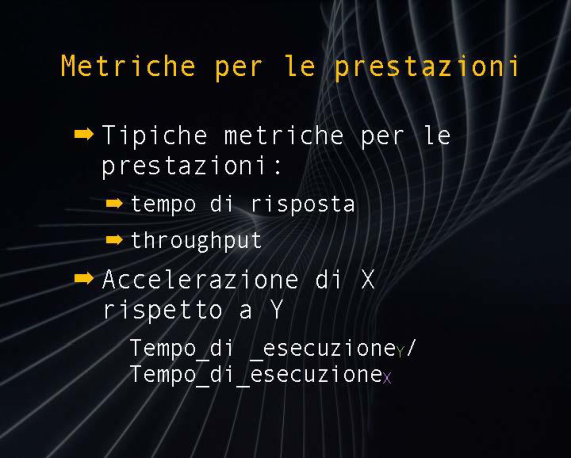
\includegraphics[width=0.40\textwidth,
                    trim=40 40 10 40, % L B R T
                    clip]
                    {images/Lez03_p03_fig_03.png}
  \caption{Misura delle prestazioni}
  \label{fig:Lez03_p03_fig_03}
\end{figure}
\FloatBarrier
\noindent

Cerchiamo di definire un metodo per procedere alla misurazione delle prestazioni.
Per molti anni si è sempre assunto un clock più veloce, una frequenza di clock più alta era indice di maggiori prestazioni.
Questo non solo non era corretto in passato ma non lo è assolutamente ora che siamo in un mondo dove ormai vige il multicore e anche all'interno della stessa instruction set architecture, cioè delLO stesso repertorio di istruzioni, come abbiamo visto, vi sono diverse implementazioni fra diversi produttori o all'interno anche dello stesso produttore.
Facciamo un esempio, fra l'architettura per PMD atom all'architettura per un desktop ci sono delle differenze sostanziali.
Se andate a vedere un'architettura Intel Phi che fondamentalmente per HPC, High Performance Computing, vi accorgete che il clock è molto più lento del normale desktop, però la macchina, cioè quel processore è sensibilmente più performante.
Quindi in linea di principio l'uso del clock come parametro di metodo è del tutto insignificante oggigiorno.

Bisogna cercare di definire qualche criterio più oggettivo per procedere alla misurazione delle prestazioni dei calcolatori.
Bisogna definire delle metriche per le prestazioni.

Tipiche metriche per le prestazioni sono:

Il \textbf{tempo di risposta}, cioè quanto tempo intercorre fra quando voi date un comando al sistema di elaborazione e quando questo vi dà la risposta.
Per esempio lanciate un programma di calcolo e dopo quanto tempo il programma di calcolo ha finito e ha prodotto il risultato.
Ha prodotto il risultato in che modo? Dipende da come voi avete programmato quel programma di calcolo, cioè se il dato deve essere visualizzato, allora magari interverrà anche la GPU che deve fare degli ulteriori calcoli. Se invece il dato deve essere archiviato su un supporto di massa, dovete considerare che all'interno della metrica delle prestazioni intercorre anche il tempo per la scrittura su un supporto di massa.
Quindi se ad esempio lo scrivete su stick USB o se lo scrivete su un disco ci saranno dei tempi diversi.
Se dovete archiviarlo su un nastro o su un supporto ottico per archiviazione, anche lì ci saranno dei tempi diversi.
Quindi il concetto di metrica deve essere olistico, non può essere legato solamente a un semplice parametro.

Altro parametro della metrica può essere il così detto \textbf{throughput}, cioè quanti eventi avvengono per unità di tempo.
Notate che tempo di risposta e throughput non sono necessariamente correlati. Perché? 
In alcuni casi si può avere un elevato throughput ma il tempo di risposta è lungo e poi tutti gli altri eventi avvengono successivamente.
Questo lo abbiamo visto anche quando parlavamo delle pipeline nel corso di primo livello.
Lì ci si accorge di come la pipeline deve essere riempita, ma una volta che la pipeline è riempita con un certo numero di colpi di clock, a un certo punto il dato viene prodotto in uscita.
Nello stesso caso anche in generale per una metrica a più alto livello, anche in questo caso il throughput può non essere direttamente correlato al tempo di risposta.
Dobbiamo decidere quindi una qualche metrica.

Definiamo quindi una accelerazione di x rispetto a y, cioè fra due diverse situazioni nel nostro sistema di elaborazione che chiameremo x e y, per esempio due versioni diverse del codice oppure due diverse implementazioni dell'hardware oppure una diversa scelta della microarchitettura o via discorrendo.

Nel nostro approccio olistico per esempio potremmo anche definire \textbf{accelerazione} di x rispetto a y, ad esempio il tempo di risposta della scrittura di un programma su un tipo di disco o di un altro tipo di disco più veloce, più veloce poi rispetto a cosa, lo definiremo. Ma in questo caso tutto il resto rimane uguale. Facciamo una scelta se usare uno dello storage a stato solito, cioè tipicamente basato su flash o un disco magnetico, in questo caso faremo una misurazione dell'accelerazione delle nostre attività considerando non più il processore. Vedete come non è importante focalizzarsi solo sul processore ma sul nostro problema.

Come si misura l'accelerazione di x rispetto a y?
Si misura in tempo, cioè tempo di esecuzione di y diviso tempo di esecuzione di x, questa è l'unica metrica che ha un senso.
L'accelerazione dei tempi di risposta lo misureremo come rapporto fra i tempi.

\FloatBarrier
\begin{figure}[H]
  \centering
  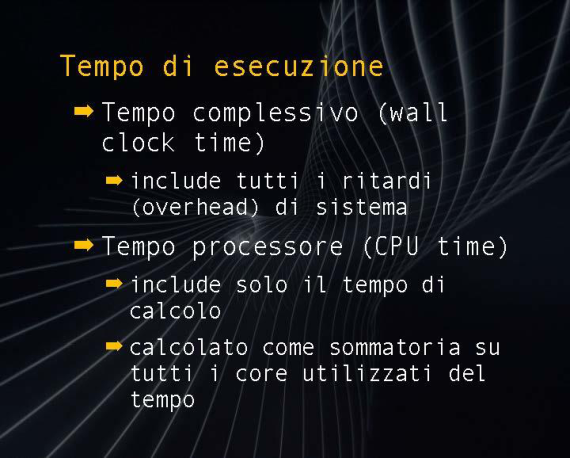
\includegraphics[width=0.40\textwidth,
                    trim=40 40 10 40, % L B R T
                    clip]
                    {images/Lez03_p03_fig_04.png}
  \caption{Tempo di esecuzione}
  \label{fig:Lez03_p03_fig_04}
\end{figure}
\FloatBarrier
\noindent

Consideriamo ora il \textbf{tempo di esecuzione}, anche in questo caso ci sono diversi modi per misurare il tempo di esecuzione.
Il tempo complessivo, quello che viene chiamato in inglese wall clock time, cioè un tempo assoluto, voi fate partire il cronometro e vedete quanto tempo ci mette, ovviamente questo cronometro è idealizzato, ma misurate fisicamente il tempo che intercorre quando date il via all'operazione che volete monitorare e il tempo in cui essa cessa.
Ad esempio quanto ci si mette a eseguire un certo programma di calcolo, una certa operazione, una certa transazione.
Questo tempo di complessivo include tutti i ritardi o overhead del sistema.

Per esempio il tempo di caricamento del programma da supporto magnetico in ram e l'esecuzione del programma e l'archiviazione su supporto magnetico dei risultati.
Questo potrebbe per esempio essere costitutivo di tutti i tempi, cioè dall'inizio alla fine.
Per esempio avete fatto una riga di un codice batch che carica il programma, che deve essere caricato dal loader, deve essere eseguito quindi sarà importante avere un disco veloce per poter leggere, abbiamo necessità di un processore veloce, di una ram veloce, un'altra volta di scrivere il dato.
Per esempio possiamo aver deciso che il dato lo andiamo a stampare su una stampante, in questo caso intercorre il tempo di scrittura della stampante perché il dispositivo di uscita è la stampante.
Se il nostro compito da eseguire è eseguire il programma, produrre per esempio una certa immagine in un certo modo e stamparla il tempo complessivo è quello che va dall'istante in cui parte l'operazione all'istante in cui è completata la stampa, quindi all'interno del nostro sistema di elaborazione vi è anche il tempo per esempio di esecuzione delle periferiche.

In altri casi si conta il \textbf{tempo processore o CPU time}, abbiamo detto che il termine CPU è spesso desueto perché aveva un senso quando c'era un singolo core, oggi giorno il termine CPU può essere un po' ingannevole, misleading in inglese e può a volte riferirsi al tempo del singolo core o al tempo di tutta l'elaborazione.
Noi cerchiamo di considerare questo prevalentemente come tempo del singolo core negli esempi che facciamo più avanti.
Questo tempo processore include solo il tempo di calcolo vero e proprio, cioè non include ad esempio il tempo necessario per caricare il programma da supporto magnetico in ram, non include i tempi per l'intercomunicazione necessari per far comunicare ad esempio il processore con una periferica, né i tempi per archiviazione dei dati, in questo caso ovviamente su un supporto di massa, è solo il tempo di calcolo vero e proprio.
Nel caso si usino più core, il tempo processore è calcolato come sommatoria dei tempi di calcolo di tutti i core utilizzati.
%%%%%%%%%%%%%%%
Ad esempio se voi avete da far girare un programma parallelo, un programma numerico, fluidodinamica, elementi finiti per qualunque motivo, differenze finite e così via discorrendo, potete ad esempio affittare l'utilizzo di centri di calcolo, ad esempio in Italia c'è il Cineca in cui voi comprate un certo numero di ore di processore.
Questo presuppone chiaramente che il programma sia paralizzabile su quel numero di core, cioè questo che comprate, e che quindi sia abbastanza invariante se lo fate girare 100 ore su 100 core o 50 ore su 200 core o 200 ore su 50 core.
Sfortunatamente questo non è il caso perché non sempre i problemi scalano così linearmente con il numero dei core, sarebbe bello se fosse vero, ma questo è un modo per contabilizzare il tempo processore e ovviamente come vi ho detto dipende dal livello di paralizzazione dell'algoritmo e non tutti gli algoritmi sono facilmente paralizzabili, alcuni non lo sono quasi per niente.

\FloatBarrier
\begin{figure}[H]
  \centering
  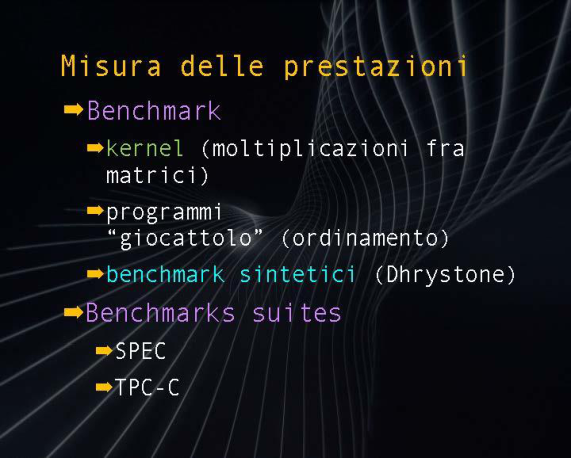
\includegraphics[width=0.40\textwidth,
                    trim=40 40 10 40, % L B R T
                    clip]
                    {images/Lez03_p03_fig_05.png}
  \caption{Misura delle prestazioni (Benchmark)}
  \label{fig:Lez03_p03_fig_05}
\end{figure}
\FloatBarrier
\noindent

Diamo altri criteri per la misura delle prestazioni.
Negli anni si sono affermati i cosiddetti benchmark, vi definirò più propriamente cosa significa benchmark più avanti.
Fra i benchmark vi sono i cosiddetti kernel, cioè ad esempio dei programmini molto semplici, per esempio per fare moltiplicazioni fra matrici, sono i nuclei di importanti programmi e generalmente riutilizzati molte volte.
Vi immaginate che quasi qualunque problema numerico alla fine è ricondotto alla moltiplicazione righe e colonne fra matrici.
È chiaro che una delle misure delle prestazioni di un calcolatore è quanto è veloce questo programma a fare delle operazioni di moltiplicazioni righe e colonna.
Questo è un bel problema perché è facilmente paralizzabile, voi potete fare in parallelo le moltiplicazioni righe e colonna per ogni colonna e quindi li potete parallelizzare abbastanza facilmente e questa può essere una delle misurazioni, cioè si va a vedere quanto tempo ci impiegano un certo numero di operazioni e moltiplicazioni fra matrici.
Sfortunatamente questo è soltanto un pezzo del problema e come vi ho detto è vero che molti problemi numerici contengono operazioni di questo tipo ma non contengono solo operazioni di questo tipo e altre categorie di problemi non le contengono quasi per niente, cioè se uno deve fare una transazione in banca e andare a interrogare un database per sapere qual è il conto corrente non è un'operazione che è facilmente riconducibile alla moltiplicazione righe e colonne come potrebbe essere per esempio l'inversione di una matrice stessa e così via.

A volte si utilizzano anche cosiddetti programmi giocattolo o toy programs in inglese, un termine che si usa, per esempio programmi inventati ad arte, degli ordinamenti di un certo numero di elementi e questo dà una qualche idea ma spesso non rappresenta un vero e proprio problema reale.

Vengono anche realizzati dei cosiddetti benchmark sintetici, nel caso dei sistemi embedded ancora è molto utilizzato il cosiddetto drystone, vedrete molte volte drystone MIPS misurati per un processore per applicazioni embedded, non è una delle migliori misure ma una misura alla fine abbastanza comune, abbastanza accettata, spesso le performance reali non corrispondono.
Quando si dice drystone MIPS si intende quante mega instruction per second, quante milioni di instructioni per secondo vengono eseguite da quelle architetture, da quel tipo di macchina.

Ormai da una ventina d'anni a questa parte si usano i cosiddetti benchmark suites, cioè sono degli insieme di programmi che rappresentano problematiche reali opportunamente combinati per rappresentare un'ampia classe di possibili utilizzi della nostra architettura di elaborazione, fra queste una di quelle che domina è la \textit{SPEC} Standard Performance Evaluation Corporation di cui parleremo un po' più avanti, ve ne è anche un'altra, TPC-C.

La definizione del dizionario di benchmark:

\FloatBarrier
\begin{figure}[H]
  \centering
  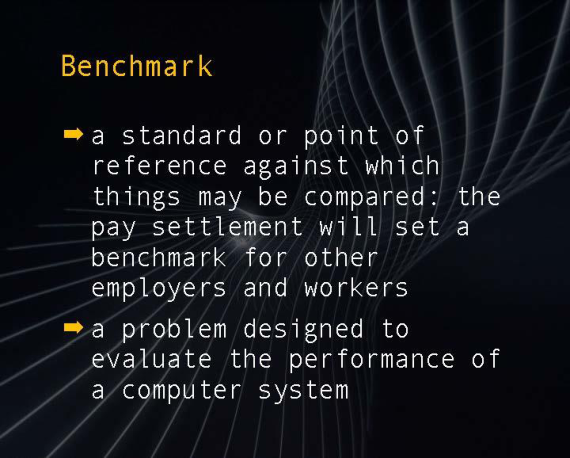
\includegraphics[width=0.40\textwidth,
                    trim=40 40 10 40, % L B R T
                    clip]
                    {images/Lez03_p03_fig_06.png}
  \caption{Misura delle prestazioni (Benchmark)}
  \label{fig:Lez03_p03_fig_06}
\end{figure}
\FloatBarrier
\noindent

è uno standard o punto di riferimento rispetto a cose che possono essere comparate.
E' allo stesso tempo uno standard o un punto di riferimento su misurazioni, ma è proprio un problema disegnato per valutare le performance, quindi le due cose sono esattamente coincidenti dal punto di vista della misurazione delle prestazioni di un sistema di elaborazione.

Andiamo a vedere alcuni benchmark suites:

\FloatBarrier
\begin{figure}[H]
  \centering
  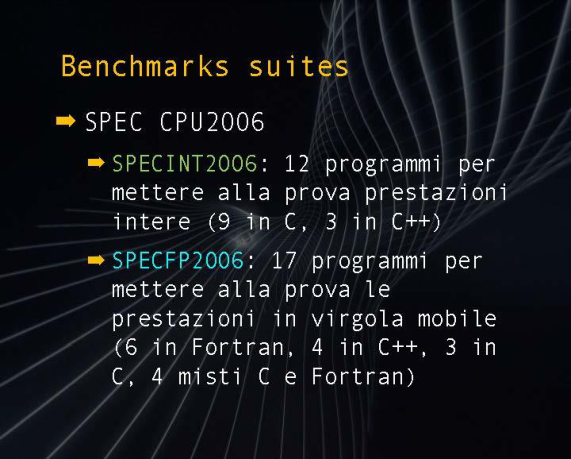
\includegraphics[width=0.40\textwidth,
                    trim=40 40 10 40, % L B R T
                    clip]
                    {images/Lez03_p04_fig_01.png}
  \caption{Misura delle prestazioni (SPECS)}
  \label{fig:Lez03_p04_fig_01}
\end{figure}
\FloatBarrier
\noindent

Si è partiti dalla metà degli anni 90 in diverse evoluzioni, quella che ancora è utilizza è la spec cpu 2006 che è rappresentata da due insiemi, la spec int 2006 fatta da 12 programmi per mettere alla prova le prestazioni intere, cioè a virgola fissa, di questi 12 programmi 9 sono scritti in linguaggio C e 3 in linguaggio C++.

Esiste anche un corrispondente spec fp 2006, sono 17 programmi per mettere a punto le prestazioni in virgola mobile da questo floating point fp nella sigla, 6 sono realizzati in Fortran, 4 in C++, 3 in C e 4 misti in C e Fortran.

L'insieme di questi programmi ogni quinquennio vengono rimodificati in base a vari criteri per cercare di rappresentare quanto meglio le performance, in questo caso di una cpu.

Come vedete si misurano separatamente le performance intere e le performance in virgola mobile.
Notate che tra le performance in virgola mobile sopravvive ancora il venerando linguaggio di programmazione Fortran che sta per formula translation introdotto negli anni 50 come grande evoluzione rispetto ai linguaggi assemblativi perché consentiva chiaramente ai programmatori una maggiore produttività.

\FloatBarrier
\begin{figure}[H]
  \centering
  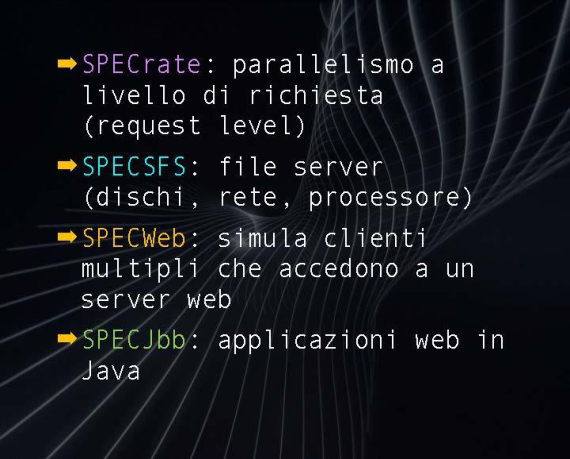
\includegraphics[width=0.40\textwidth,
                    trim=40 40 10 40, % L B R T
                    clip]
                    {images/Lez03_p04_fig_02.png}
  \caption{Misura delle prestazioni (SPECS II)}
  \label{fig:Lez03_p04_fig_02}
\end{figure}
\FloatBarrier
\noindent

Nel caso si voglia lavorare a un livello più alto, esiste la spec rate che misura il parallelismo a livello di richiesta, il cosiddetto request level parallelism.

Poi esiste una spec fs che sta per file server e quindi si misurano le performance complessive di dischi della rete di interconnessione del processore, quindi non più soltanto del processore.

Notate che questi due benchmark suites, in realtà non è un singola programma, sono complementari a quelle della cpu, quindi dipende da quale l'obiettivo per cui voi dovete disegnare o acquistare un'unità di elaborazione.
Se dovete fare solamente del cosiddetto number crunching, vi preoccuperete prevalentemente dello spec fp perché quella vi dà una misura più fedele di un problema di calcolo numerico tipicamente fatto in virgola mobile.

Se dovete dimensionare un server, per esempio, ftp, file transfer protocol, andrete a valutarlo rispetto allo spec fs.
Nel caso in cui dovete dimensionare un server di tipo web, una delle misure può essere data dallo spec web che simula diversi clients o clienti multipli che accedono a un server web.
Notate che le cose sono sensibilmente diverse, fra gestire semplicemente un flusso di dati o gestire, per esempio, quindi come un file server che non fa più che leggere un disco e mettere sulla rete, un server web svolge anche delle funzioni un po' più complicate.
E infine vi menziono lo spec jbb che serve a misurare le performance della vostra unità di elaborazione rispetto ad applicazioni web scritte tutte in java.
Molte applicazioni sono scritte in java, vuoi per la sua efficienza, vuoi per la sua indipendenza, ma soprattutto perché esistono dei just-in-time compiler che rendono l'esecuzione di java abbastanza efficiente su una molteplicità di piattaforme differenti.

\subsection{Principi di progetto}

\FloatBarrier
\begin{figure}[H]
  \centering
  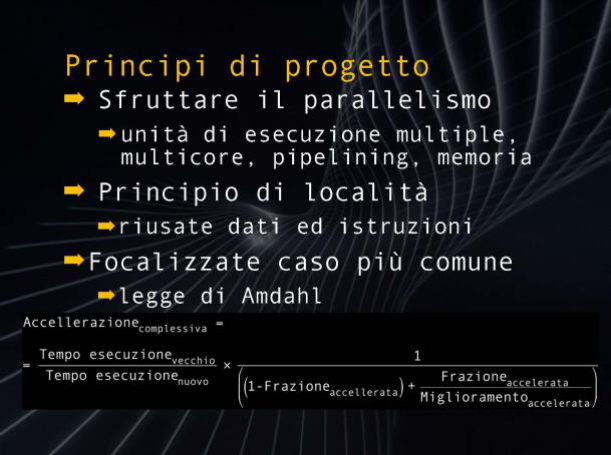
\includegraphics[width=0.80\textwidth,
                    trim=10 40 10 40, % L B R T
                    clip]
                    {images/Lez03_p04_fig_03.png}
  \caption{Principi di progetto}
  \label{fig:Lez03_p04_fig_03}
\end{figure}
\FloatBarrier
\noindent

Passiamo ora a definire alcuni principi generali di progetto unità di elaborazione.
Ovviamente occorre sfruttare il parallelismo al massimo perché non è più possibile invocare semplicemente l'aumento di frequenza grazie alla legge di Moore.
Come vi ho detto, ormai da un po' di anni il parallelismo è indispensabile per migliorare le performance.
Quindi consideremo le unità di esecuzione multiple, multicore, pipelining, memoria, quindi i livelli di parallelismo sia all'interno del singolo chip, del singolo core, che fra diversi core e anche fra diversi chip.

Cercheremo di sfruttare dei principi di località, cioè quando andiamo a gestire i nostri programmi cercheremo di avere dati locali e istruzioni locali in maniera da sfruttare al meglio le gerarchie di cache.

Cercheremo di ottimizzare il nostro problema focalizzandoci sul caso più comune. Questo è importante, viene codificato nella cosiddetta legge di Amdahl che vedete scritta qui brevemente.

L'accelerazione complessiva di un'unità di elaborazione è misurata come il rapporto fra il tempo di esecuzione prima della modifica diviso il tempo di esecuzione dopo la modifica, moltiplicato per una frazione che a denominatore contiene uno meno la frazione del codice accelerata più la frazione accelerata diviso il miglioramento della frazione accelerata.
Sembra complicato ma questa è quella che viene chiamata in inglese the law of diminishing return, cioè la legge del ritorno che diminuisce.

\FloatBarrier
\begin{figure}[H]
  \centering
  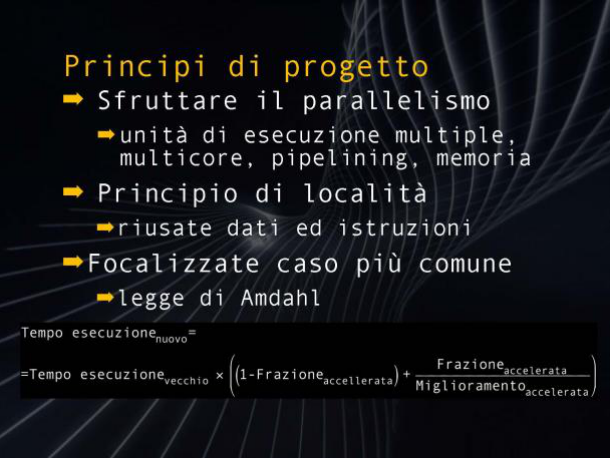
\includegraphics[width=0.80\textwidth,
                    trim=10 40 10 40, % L B R T
                    clip]
                    {images/Lez03_p04_fig_04.png}
  \caption{Principi di progetto}
  \label{fig:Lez03_p04_fig_04}
\end{figure}
\FloatBarrier
\noindent

Un'altra formulazione della legge è data come tempo di esecuzione nuovo è uguale al tempo di esecuzione vecchio per uno meno la frazione del codice accelerata più la frazione accelerata diviso il miglioramento.
Questo può essere il codice ma anche in una ottica di sistema tutti i pezzi che contribuiscono al rallentamento.
Per esempio i tempi di accesso su un disco entrano nel tempo complessivo, quindi se voi avete molte transazioni su disco vi converrà a cercare un disco più veloce, ad esempio passare su dischi a stato solido.
Se invece avete un problema maggiormente focalizzato sul tempo di calcolo, gli accessi ai supporti di massa possono non essere determinanti quindi è inutile investire sui supporti di massa se è tutto legato al calcolo.
Se il collo di bottiglia è la memoria cercherete di avere memorie più veloci e così via.
Ma sappiate che non riuscite mai ad avere un miglioramento maggiore della percentuale su cui agite.

\FloatBarrier
\begin{figure}[H]
  \centering
  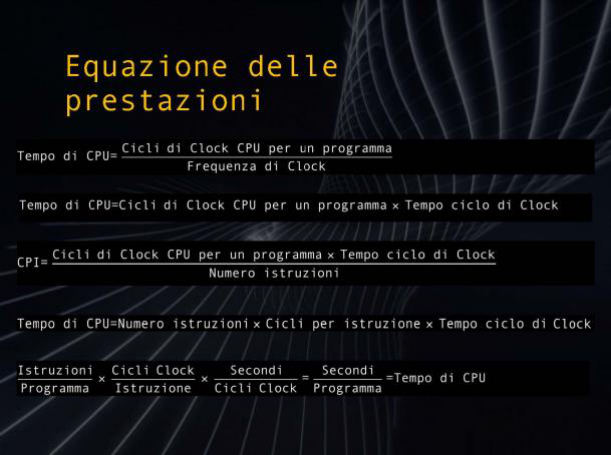
\includegraphics[width=0.80\textwidth,
                    trim=10 40 10 40, % L B R T
                    clip]
                    {images/Lez03_p04_fig_06.png}
  \caption{Equazione delle prestationi}
  \label{fig:Lez03_p04_fig_06}
\end{figure}
\FloatBarrier
\noindent

Guardiamo alcune delle equazioni delle prestazioni: 

tempo di CPU il numero di cicli di clock diviso la frequenza di clock, il tempo di CPU può anche essere scritto come cicli di clock della CPU per un programma per il tempo del ciclo di clock, 

il cosiddetto clock per instruction il numero di cicli di clock della CPU per un programma moltiplicato il tempo di ciclo di clock e diviso il numero delle istruzioni spesso il clock per instruction era un numero maggiore di uno oggi con il parallelismo possiamo pensare che sia anche un numero minore di uno.

Il tempo di CPU è calcolato come il numero delle istruzioni per i cicli per istruzione per il tempo di ciclo di clock ed infine per ottenere il tempo di CPU si considera il rapporto tra istruzioni per programma, il numero di cicli di clock per istruzioni, quanti secondi per ciclo di clock e si trova esattamente quanti secondi per svolgere lo stesso programma cioè il tempo di CPU.

\FloatBarrier
\begin{figure}[H]
  \centering
  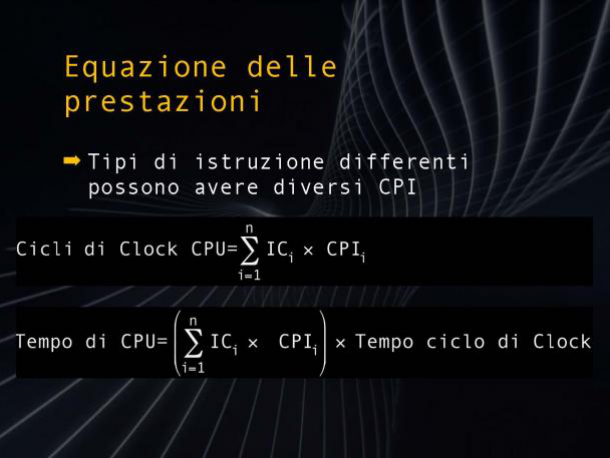
\includegraphics[width=0.60\textwidth,
                    trim=10 40 10 40, % L B R T
                    clip]
                    {images/Lez03_p04_fig_05.png}
  \caption{Equazioni delle prestazioni}
  \label{fig:Lez03_p04_fig_05}
\end{figure}
\FloatBarrier
\noindent

Un ulteriore tipo di istruzioni differenti notate che possono avere diverse clock per instructions, in generale i cicli di clock di un programma sono dati dalla sommatoria delle istruzioni moltiplicate per i cicli di clock per istruzione quindi il tempo di CPU complessivo è quindi dato da questa sommatoria moltiplicata per il tempo di ciclo di clock che in questo caso assumiamo costante.

Infine vi do l'ultimo spunto della riflessione e vi invito a riflettere se un processore multicore è sempre più veloce di un single core e quali sono gli elementi che limitano l'aumento di velocità di un multicore.